% =============================================================================
% Chest Xpert AI - Multi-Label Chest Pathology Classifier
% Academic Product (PAC) - Scientific Article
% =============================================================================
\documentclass[9pt, twocolumn, a4paper]{extarticle}

% --- Core Packages ---
\usepackage[utf8]{inputenc}
\usepackage[T1]{fontenc}

% Use spanish for captions and content
\usepackage[spanish]{babel}

% Layout and margins
\usepackage[top=2cm, bottom=2cm, left=1.8cm, right=1.8cm]{geometry}

% Reduce whitespace around sections and floats
\usepackage{titlesec}
\titlespacing*{\section}{0pt}{6pt plus 2pt minus 2pt}{2pt plus 1pt}
\titlespacing*{\subsection}{0pt}{4pt plus 2pt minus 1pt}{1pt plus 1pt}

% Graphics and figures
\usepackage{graphicx}
\usepackage{float}
\usepackage[font=small, labelfont=bf, skip=4pt]{caption}

% Tables
\usepackage{booktabs}
\usepackage{tabularx}
\usepackage{array}
\setlength{\tabcolsep}{4pt}

% Lists (compact)
\usepackage{enumitem}
\setlist{nosep, leftmargin=*, topsep=2pt, parsep=0pt, itemsep=1pt}

% Mathematics and symbols
\usepackage{amsmath}
\usepackage{amssymb}

% Colors and links
\usepackage{xcolor}
\usepackage[hidelinks]{hyperref}
\usepackage{url}

% Bibliography
\usepackage[numbers, sort&compress]{natbib}
\setlength{\bibsep}{2pt}

% Headers and footers
\usepackage{fancyhdr}
\pagestyle{fancy}
\fancyhf{}
\fancyhead[L]{\footnotesize Chest Xpert AI - Clasificaci\'on de Patolog\'ias Tor\'acicas}
\fancyhead[R]{\footnotesize \thepage}
\renewcommand{\headrulewidth}{0.4pt}

% Tighter column separation
\setlength{\columnsep}{0.6cm}

% Prevent vertical stretching between paragraphs to fill columns
\raggedbottom

% Reduce space before/after floats
\setlength{\floatsep}{2pt}
\setlength{\textfloatsep}{4pt}
\setlength{\intextsep}{2pt}
\setlength{\abovecaptionskip}{3pt}
\setlength{\belowcaptionskip}{0pt}

% Reduce abstract spacing
\usepackage{abstract}
\setlength{\absleftindent}{0pt}
\setlength{\absrightindent}{0pt}
\renewcommand{\abstractnamefont}{\normalfont\bfseries}
\renewcommand{\abstracttextfont}{\normalfont\small}

% =============================================================================
% DOCUMENT METADATA
% =============================================================================
\title{
    \vspace{-2cm}
    \large\textbf{Chest Xpert AI: Clasificaci\'on Autom\'atica Multi-Etiqueta de Patolog\'ias Tor\'acicas mediante Deep Learning con Transfer Learning Especializado} \\[0.1cm]
    \small\normalfont Producto Acad\'emico --- Aprendizaje Autom\'atico --- Maestr\'ia en Inteligencia Artificial
}

\author{
    \textbf{Angel Hincho Jove}\textsuperscript{1} \quad
    \textbf{Angel Espinoza Julca}\textsuperscript{2} \quad
    \textbf{Juan Martinez Yupanqui}\textsuperscript{3} \\[0.1cm]
    \small\textsuperscript{1}\textit{Universidad Continental, Facultad de Ingenier\'ia} \\
    \small\texttt{72190199@continental.edu.pe}\textsuperscript{1} \quad
    \small\texttt{42702445@continental.edu.pe}\textsuperscript{2} \quad
    \small\texttt{08646067@continental.edu.pe}\textsuperscript{3}
}

\date{\vspace{-0.3cm}\small\today}

% =============================================================================
% DOCUMENT START
% =============================================================================
\begin{document}

\twocolumn[
    \maketitle
    \vspace{-0.6cm}
    \begin{@twocolumnfalse}
        % =============================================================================
% RESUMEN
% =============================================================================
\begin{abstract}
\noindent
\textbf{Resumen.}
La radiograf\'ia de t\'orax representa el 40\% del volumen global de imagen diagn\'ostica, pero dos tercios de la poblaci\'on mundial carecen de acceso a servicios de radiolog\'ia y los radi\'ologos disponibles enfrentan tasas de error del 3--5\% agravadas por fatiga. El presente trabajo desarrolla un sistema de clasificaci\'on autom\'atica multi-etiqueta de cinco patolog\'ias tor\'acicas urgentes (Cardiomegaly, Edema, Consolidation, Atelectasis, Pleural Effusion) mediante Deep Learning con transfer learning especializado. Utilizando el dataset CheXpert (224,316 radiograf\'ias, Stanford University) y un backbone DenseNet121 preentrenado en m\'as de 500,000 radiograf\'ias reales (TorchXRayVision), se alcanz\'o un AUC de 0.869 [IC 95\%: 0.844--0.893], mejorando en 8.4\% al baseline con ImageNet. El modelo fue validado externamente contra NIH ChestX-ray14 (ca\'ida de 7.2\%), auditado por equidad de g\'enero (gap de 9.2\% en Atelectasis), calibrado mediante temperature scaling, y su interpretabilidad verificada con Grad-CAM descartando shortcut learning. Se export\'o a formato ONNX con normalizaci\'on embebida para inferencia en $\sim$20ms, eliminando training-serving skew. El sistema se propone como herramienta de triaje bajo supervisi\'on humana obligatoria, con un impacto estimado de 5x en capacidad diagn\'ostica y ROI de 24x, alineado con los marcos regulatorios FDA, AI Act europeo y las recomendaciones de la OMS.

\vspace{0.3cm}
\noindent
\textbf{Palabras clave:} Deep Learning, radiograf\'ias de t\'orax, clasificaci\'on multi-etiqueta, transfer learning, CheXpert, TorchXRayVision, ONNX, explicabilidad (Grad-CAM), equidad algor\'itmica, triaje autom\'atico.
\end{abstract}

    \end{@twocolumnfalse}
    \vspace{0.2cm}
]

% --- Sections ---
% =============================================================================
% 1. INTRODUCCION / DEFINICION DEL PROBLEMA
% =============================================================================
\section{Introducci\'on}
\label{sec:introduction}

\subsection{Contexto del problema}

La radiograf\'ia de t\'orax es el examen de imagen diagn\'ostica m\'as solicitado a nivel mundial, representando aproximadamente el 40\% de los 3.6 mil millones de estudios de imagen anuales \cite{who2016xray, ahmad2023cxr}. A pesar de este volumen, dos tercios de la poblaci\'on mundial carecen de acceso a servicios b\'asicos de radiolog\'ia \cite{who2023imaging}, y la fuerza laboral disponible enfrenta d\'eficits estructurales: el Reino Unido reporta un d\'eficit del 29\% de radi\'ologos consultores, proyectado al 39\% para 2029 \cite{rcr2025census}, mientras que pa\'ises de ingresos bajos operan con ratios de hasta 1 radi\'ologo por mill\'on de habitantes frente a aproximadamente 100 por mill\'on en naciones de altos ingresos \cite{mollura2020ai}.

Bajo estas condiciones, los radi\'ologos deben sostener ritmos de interpretaci\'on de una imagen cada 3--4 segundos durante turnos de 8 horas \cite{mcdonald2015workload}, generando una tasa basal de error diagn\'ostico del 3--5\% que escala hasta aproximadamente 30\% al evaluar ex\'amenes con hallazgos anormales \cite{bruno2015error, brady2017error}. La fatiga por turnos extendidos agrava este riesgo, con errores m\'edicos ocurriendo 12.1\% m\'as frecuentemente durante turnos nocturnos y rotativos \cite{ahrq2024fatigue}. Solo en Inglaterra, cerca de un mill\'on de resultados de imagen se retrasaron m\'as de un mes en 2025 \cite{rcr2025census}.

\subsection{La IA como soluci\'on potencial}

El Deep Learning aplicado a radiograf\'ias de t\'orax ha demostrado rendimiento a nivel de radi\'ologo desde que CheXNet alcanz\'o F1 = 0.435 frente a F1 = 0.387 del radi\'ologo promedio en detecci\'on de neumon\'ia \cite{rajpurkar2017chexnet}. M\'as recientemente, el ensayo cl\'inico aleatorizado MASAI demostr\'o una reducci\'on del 44\% en la carga de doble lectura sin comprometer las tasas de detecci\'on de c\'ancer en 80,000 pacientes \cite{lang2023masai}, y estudios prospectivos muestran una reducci\'on del 17.6\% en el tiempo de lectura para radiograf\'ias normales con asistencia de IA \cite{shin2023ai}. Sin embargo, revisiones metodol\'ogicas cr\'iticas han demostrado que 0 de m\'as de 300 modelos publicados de COVID-19 en CXR fueron cl\'inicamente \'utiles debido a fugas de datos y falta de validaci\'on externa \cite{roberts2021pitfalls}, subrayando la necesidad de evaluaci\'on rigurosa.

Adem\'as, persisten sesgos demogr\'aficos documentados: clasificadores de IA entrenados en CheXpert, MIMIC-CXR y NIH ChestX-ray14 subdiagnostican sistem\'aticamente a pacientes femeninas, afrodescendientes e hispanas en hasta 9--10 puntos porcentuales \cite{seyyedkalantari2021bias}, y el desbalance de g\'enero en datasets de entrenamiento produce clasificadores con AUC significativamente menor para el grupo subrepresentado \cite{larrazabal2020gender}. Estos hallazgos exigen que cualquier modelo orientado cl\'inicamente incluya auditor\'ia de equidad y verificaci\'on de interpretabilidad.

\subsection{Soluci\'on propuesta}

Se desarrolla un sistema de clasificaci\'on multi-etiqueta basado en Deep Learning que detecta simult\'aneamente cinco patolog\'ias tor\'acicas urgentes---Cardiomegaly, Edema, Consolidation, Atelectasis y Pleural Effusion---a partir de radiograf\'ias frontales de t\'orax. El sistema utiliza el dataset CheXpert (224,316 radiograf\'ias de 65,240 pacientes) \cite{irvin2019chexpert} con un backbone DenseNet121 preentrenado en m\'as de 500,000 radiograf\'ias reales mediante TorchXRayVision \cite{cohen2022torchxrayvision}, y est\'a dise\~nado como herramienta de triaje y priorizaci\'on para radi\'ologos, no como reemplazo.

\subsection{Objetivo}

Aplicar un modelo de Aprendizaje Autom\'atico (red neuronal convolucional con transfer learning especializado) para resolver la tarea de clasificaci\'on multi-etiqueta de patolog\'ias tor\'acicas, evaluando su rendimiento, generalizaci\'on a datos externos, interpretabilidad mediante Grad-CAM, equidad de g\'enero e impacto potencial en la eficiencia operativa hospitalaria.

% =============================================================================
% 2. PREPARACION Y LIMPIEZA DE DATOS
% =============================================================================
\section{Preparaci\'on y limpieza de datos}
\label{sec:data-preparation}

\subsection{Selecci\'on del dataset}

Se utiliz\'o CheXpert (Chest eXpert), un dataset a gran escala publicado por la Universidad de Stanford que contiene 224,316 radiograf\'ias de t\'orax de 65,240 pacientes \cite{irvin2019chexpert}. El dataset fue seleccionado por su escala suficiente para entrenar redes profundas, su anotaci\'on multi-etiqueta con manejo expl\'icito de incertidumbre, su posici\'on como benchmark est\'andar con leaderboard p\'ublico, y su acceso abierto v\'ia Kaggle. La documentaci\'on estructurada del dataset (datasheet) fue publicada por \cite{garbin2021datasheet}.

\subsection{Estructuraci\'on seg\'un Tidy Data}

El dataset fue estructurado siguiendo los tres principios can\'onicos de Tidy Data \cite{wickham2014tidy}: cada variable forma una columna (5 columnas binarias de patolog\'ia, m\'as path y metadatos), cada observaci\'on forma una fila (una radiograf\'ia), y todos los valores son consistentes (Float32, sin NaN, sin tipos mixtos). Esta estructuraci\'on garantiza reproducibilidad y compatibilidad con el pipeline de PyTorch DataLoader.

\subsection{Pipeline de preprocesamiento}

El preprocesamiento sigui\'o las pr\'acticas dominantes del campo \cite{calli2021deep}. La Tabla~\ref{tab:pipeline} resume los pasos aplicados:

\begin{table}[H]
\centering
\caption{Pipeline de preprocesamiento aplicado.}
\label{tab:pipeline}
\small
\begin{tabular}{clp{3.2cm}}
\toprule
\textbf{\#} & \textbf{Paso} & \textbf{Justificaci\'on} \\
\midrule
1 & U-Zeros        & Incertidumbre $\to$ 0 (baseline conservadora \cite{irvin2019chexpert}) \\
2 & Imputaci\'on NaN & NaN $\to$ 0 (no mencionado = ausente) \\
3 & Filtro frontal & Eliminar vistas laterales ($\sim$20\% del dataset) \\
4 & Excluir sexo   & V de Cram\'er $<$ 0.1; riesgo de sesgo \cite{gichoya2022ai} \\
5 & Normalizar XRV & Rango $[-1024, 1024]$ \cite{cohen2022torchxrayvision} \\
6 & Augmentation   & Flip-H + rotaci\'on $\pm$10\textdegree \\
\bottomrule
\end{tabular}
\end{table}

\textbf{Manejo de etiquetas inciertas.} CheXpert introduce etiquetas de incertidumbre (-1) que admiten m\'ultiples estrategias. El paper original \cite{irvin2019chexpert} demostr\'o que la estrategia \'optima depende de la patolog\'ia: U-Ones para Atelectasis/Edema, U-MultiClass para Cardiomegaly/Pleural Effusion. Trabajos posteriores \cite{pham2021interpreting} alcanzaron AUC = 0.940 mediante Label Smoothing Regularization. Se eligi\'o U-Zeros como baseline conservadora y reproducible, reconociendo que es sub\'optima para Atelectasis y Edema.

\textbf{Filtrado de vistas.} Se conservaron \'unicamente vistas frontales (AP/PA), eliminando $\sim$32,000 vistas laterales. Esta decisi\'on se alinea con la pr\'actica est\'andar del campo \cite{calli2021deep}: mezclar vistas obliga al modelo a aprender dos ``lenguajes visuales'' distintos, reduciendo el rendimiento en $\sim$1--2 puntos AUC.

\textbf{Normalizaci\'on.} Se aplic\'o la normalizaci\'on est\'andar de TorchXRayVision \cite{cohen2022torchxrayvision}: $(2 \times (img/255) - 1) \times 1024$, mapeando p\'ixeles al rango $[-1024, 1024]$. Esta normalizaci\'on es obligatoria para preservar la compatibilidad con los pesos preentrenados sobre $\sim$500K radiograf\'ias.

\textbf{Resoluci\'on.} Se utiliz\'o 224$\times$224 p\'ixeles, compatible con los pesos DenseNet121 de TorchXRayVision. Seg\'un \cite{sabottke2020resolution}, el AUC se estabiliza entre 256--320 para las patolog\'ias de competencia; 224 es suficiente para Cardiomegaly, Edema y Pleural Effusion.

\textbf{Data augmentation.} Se aplicaron \'unicamente augmentations geom\'etricas conservadoras: flip horizontal (p=0.5) y rotaci\'on $\pm$10\textdegree. No se utiliz\'o flip vertical por su incompatibilidad anat\'omica con la orientaci\'on tor\'acica \cite{calli2021deep}.

\textbf{Split de datos.} Se utiliz\'o el split oficial por paciente \cite{garbin2021datasheet} ($\sim$191K entrenamiento, 234 validaci\'on), que previene data leakage entre estudios del mismo paciente \cite{rouzrokh2022mitigating}. Se reconoce la limitaci\'on del tama\~no reducido del validation set (IC 95\% del AUC $\sim\pm$0.03--0.05), por lo que se complement\'o con validaci\'on externa (Secci\'on~\ref{sec:results}).

Resultado final: $\sim$190,000 im\'agenes frontales de entrenamiento y $\sim$200 de validaci\'on, en formato tensor $(1, 224, 224)$, float32.

% =============================================================================
% 3. ANALISIS EXPLORATORIO DE DATOS
% =============================================================================
\section{An\'alisis exploratorio}
\label{sec:exploratory-analysis}

\subsection{Distribuci\'on de patolog\'ias}

El an\'alisis de prevalencia revel\'o un desbalance significativo entre clases (Figura~\ref{fig:prevalence}): Pleural Effusion presenta la mayor prevalencia ($\sim$40\%), seguida de Atelectasis ($\sim$30\%), Cardiomegaly ($\sim$15\%), Edema ($\sim$12\%) y Consolidation ($\sim$5\%). Este desbalance justifica el uso de AUC-ROC como m\'etrica principal, ya que es insensible al umbral de decisi\'on y al desbalance de clases---criterio adoptado por la competencia oficial CheXpert \cite{irvin2019chexpert}.

\begin{figure}[H]
    \centering
    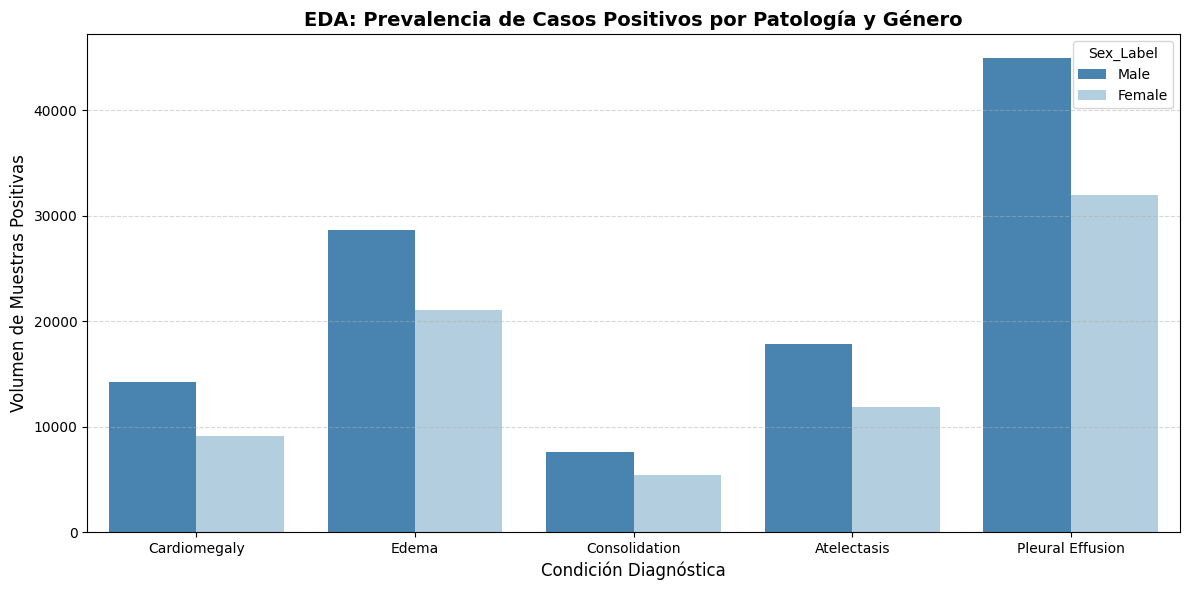
\includegraphics[width=\columnwidth]{figures/pathology-prevalence-by-gender.png}
    \caption{Prevalencia de casos positivos por patolog\'ia y g\'enero en el conjunto de entrenamiento ($\sim$190k im\'agenes frontales).}
    \label{fig:prevalence}
\end{figure}

La co-ocurrencia de patolog\'ias (un paciente puede presentar m\'ultiples condiciones simult\'aneamente) justifica la elecci\'on de clasificaci\'on multi-etiqueta con activaci\'on Sigmoid independiente por clase, en lugar de Softmax excluyente.

\subsection{An\'alisis estad\'istico: variable sexo}

La composici\'on demogr\'afica del dataset muestra un ratio Male/Female de 1.42:1 (112,151 hombres vs 78,875 mujeres), consistente con la poblaci\'on hospitalaria de Stanford. Para determinar si el sexo biol\'ogico deb\'ia incluirse como predictor, se realiz\'o un an\'alisis de independencia mediante test Chi-cuadrado y tama\~no del efecto (V de Cram\'er) para cada patolog\'ia (Tabla~\ref{tab:chi2}).

\begin{table}[H]
\centering
\caption{An\'alisis de independencia entre sexo y patolog\'ia.}
\label{tab:chi2}
\small
\begin{tabular}{lccc}
\toprule
\textbf{Patolog\'ia} & \textbf{p-value} & \textbf{V de Cram\'er} & \textbf{Efecto} \\
\midrule
Cardiomegaly     & $<$ 0.05 & 0.06 & Negligible \\
Edema            & $<$ 0.05 & 0.04 & Negligible \\
Consolidation    & $<$ 0.05 & 0.02 & Negligible \\
Atelectasis      & $<$ 0.05 & 0.03 & Negligible \\
Pleural Effusion & $<$ 0.05 & 0.05 & Negligible \\
\bottomrule
\end{tabular}
\end{table}

Con $N > 200{,}000$ muestras, la significancia estad\'istica ($p < 0.05$) no implica significancia pr\'actica. Los valores de V de Cram\'er ($< 0.1$) confirman que el sexo explica menos del 1\% de la varianza en la presencia de patolog\'ias.

\subsection{Decisi\'on: exclusi\'on de la variable sexo}

Se decidi\'o excluir la variable sexo del modelo por cuatro razones fundamentales:

\begin{enumerate}
    \item \textbf{Efecto pr\'actico negligible}: V de Cram\'er $< 0.1$ para todas las patolog\'ias.
    \item \textbf{Riesgo de sesgo algor\'itmico}: incluir el sexo puede perpetuar disparidades diagn\'osticas. \cite{seyyedkalantari2021bias} demostraron que modelos entrenados en CheXpert subdiagnostican sistem\'aticamente a pacientes femeninas incluso sin sexo como input.
    \item \textbf{Redundancia}: \cite{jabbour2020shortcuts} y \cite{gichoya2022ai} demostraron que las CNNs pueden predecir sexo desde la imagen sola con AUC $>$ 0.96, lo que indica que la red ya tiene acceso impl\'icito a esta informaci\'on a trav\'es de marcadores anat\'omicos.
    \item \textbf{Simplicidad}: un modelo solo-imagen es m\'as f\'acil de desplegar en producci\'on y no requiere metadatos cl\'inicos del paciente.
\end{enumerate}

Esta decisi\'on se alinea con la recomendaci\'on de \cite{larrazabal2020gender}, quienes demostraron que el desbalance de g\'enero en datasets de CXR produce clasificadores sesgados independientemente de incluir sexo como variable. La limitaci\'on reconocida es que excluir la variable no elimina el sesgo---solo impide medirlo directamente---por lo que se implement\'o una auditor\'ia de equidad desagregada por sexo en la fase de evaluaci\'on (Secci\'on~\ref{sec:ethics}).

\begin{figure}[H]
    \centering
    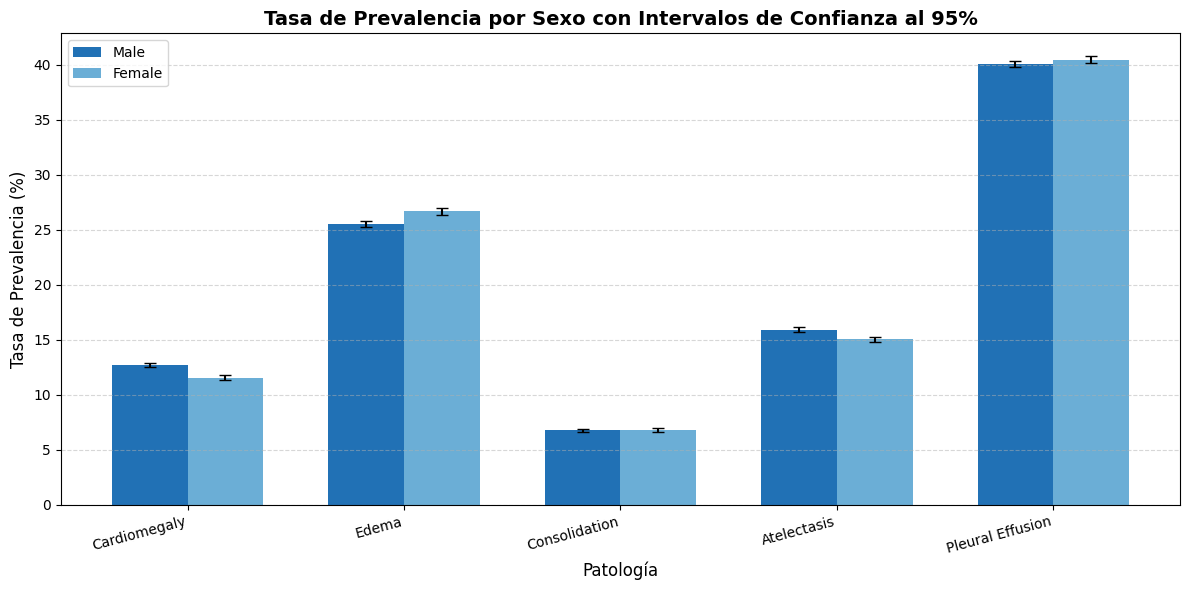
\includegraphics[width=\columnwidth]{figures/prevalence-rate-by-sex-ci95.png}
    \caption{Tasa de prevalencia por sexo con intervalos de confianza al 95\%. Las diferencias son estad\'isticamente significativas pero pr\'acticamente negligibles (V de Cram\'er $<$ 0.1).}
    \label{fig:prevalence-sex}
\end{figure}

% =============================================================================
% 4. MODELADO PREDICTIVO
% =============================================================================
\section{Modelado predictivo}
\label{sec:modeling}

\subsection{Justificaci\'on del modelo}

Se seleccion\'o una red neuronal convolucional (CNN) con transfer learning por las razones presentadas en la Tabla~\ref{tab:justification}:

\begin{table}[H]
\centering
\caption{Justificaci\'on de decisiones de modelado.}
\label{tab:justification}
\small
\begin{tabular}{lp{4cm}}
\toprule
\textbf{Decisi\'on} & \textbf{Justificaci\'on} \\
\midrule
Deep Learning    & Im\'agenes de alta dimensionalidad ($224{\times}224$) \\
DenseNet121      & 7M par\'ametros, est\'andar en radiolog\'ia \cite{huang2017densenet} \\
TorchXRayVision  & Preentrenado en 500k+ radiograf\'ias \cite{cohen2022torchxrayvision} \\
Backbone congelado & Previene olvido catastr\'ofico \\
BCELoss+Sigmoid  & Multi-etiqueta (patolog\'ias independientes) \\
Early Stopping   & Previene sobreajuste \cite{prechelt1998early} \\
\bottomrule
\end{tabular}
\end{table}

\subsection{Arquitectura del modelo}

La arquitectura consiste en un backbone TorchXRayVision DenseNet121 congelado seguido de una cabeza clasificadora entrenada desde cero. Entrada: imagen en escala de grises $(1, 224, 224)$ normalizada a $[-1024, 1024]$. Salida: 5 probabilidades independientes $\in [0, 1]$, una por patolog\'ia (activaci\'on Sigmoid para independencia multi-etiqueta).

\subsection{Configuraci\'on de entrenamiento}

\begin{itemize}
    \item \textbf{Optimizador}: Adam ($lr = 0.001$)
    \item \textbf{Loss}: Binary Cross-Entropy (BCELoss)
    \item \textbf{M\'etrica}: MultilabelAUROC (promedio macro)
    \item \textbf{\'Epocas}: m\'aximo 20 (Early Stopping, patience = 5)
    \item \textbf{Batch size}: 32
    \item \textbf{GPU}: NVIDIA A100-SXM4-40GB
\end{itemize}

\subsection{B\'usqueda de hiperpar\'ametros}

Se realiz\'o una b\'usqueda exhaustiva (Grid Search) mediante W\&B Sweeps \cite{wandb2020} con 9 configuraciones ($3 \times 3$: learning rate $\in \{0.0001, 0.001, 0.01\}$, \'epocas $\in \{5, 10, 20\}$). La mejor configuraci\'on fue $lr = 0.001$, 5 \'epocas, con AUC = 0.8745.

\subsection{Evaluaci\'on del rendimiento}

La Tabla~\ref{tab:results-models} presenta la comparativa de rendimiento entre configuraciones:

\begin{table}[H]
\centering
\caption{Comparativa de rendimiento entre modelos.}
\label{tab:results-models}
\small
\begin{tabular}{llcc}
\toprule
\textbf{Modelo} & \textbf{Backbone} & \textbf{AUC} & \textbf{\'Epocas} \\
\midrule
TensorFlow (baseline) & ImageNet & 0.806 & 8 \\
PyTorch + ImageNet & ImageNet & 0.784 & 3 \\
\textbf{PyTorch + XRV} & \textbf{TorchXRayVision} & \textbf{0.869} & \textbf{6} \\
Sweep best & TorchXRayVision & 0.874 & 5 \\
Fine-tuning & XRV (denseblock4) & 0.868 & --- \\
\bottomrule
\end{tabular}
\end{table}

El intervalo de confianza obtenido mediante bootstrap (1000 iteraciones) fue: AUC = 0.8690 [IC 95\%: 0.8439 -- 0.8931].

\begin{figure}[H]
    \centering
    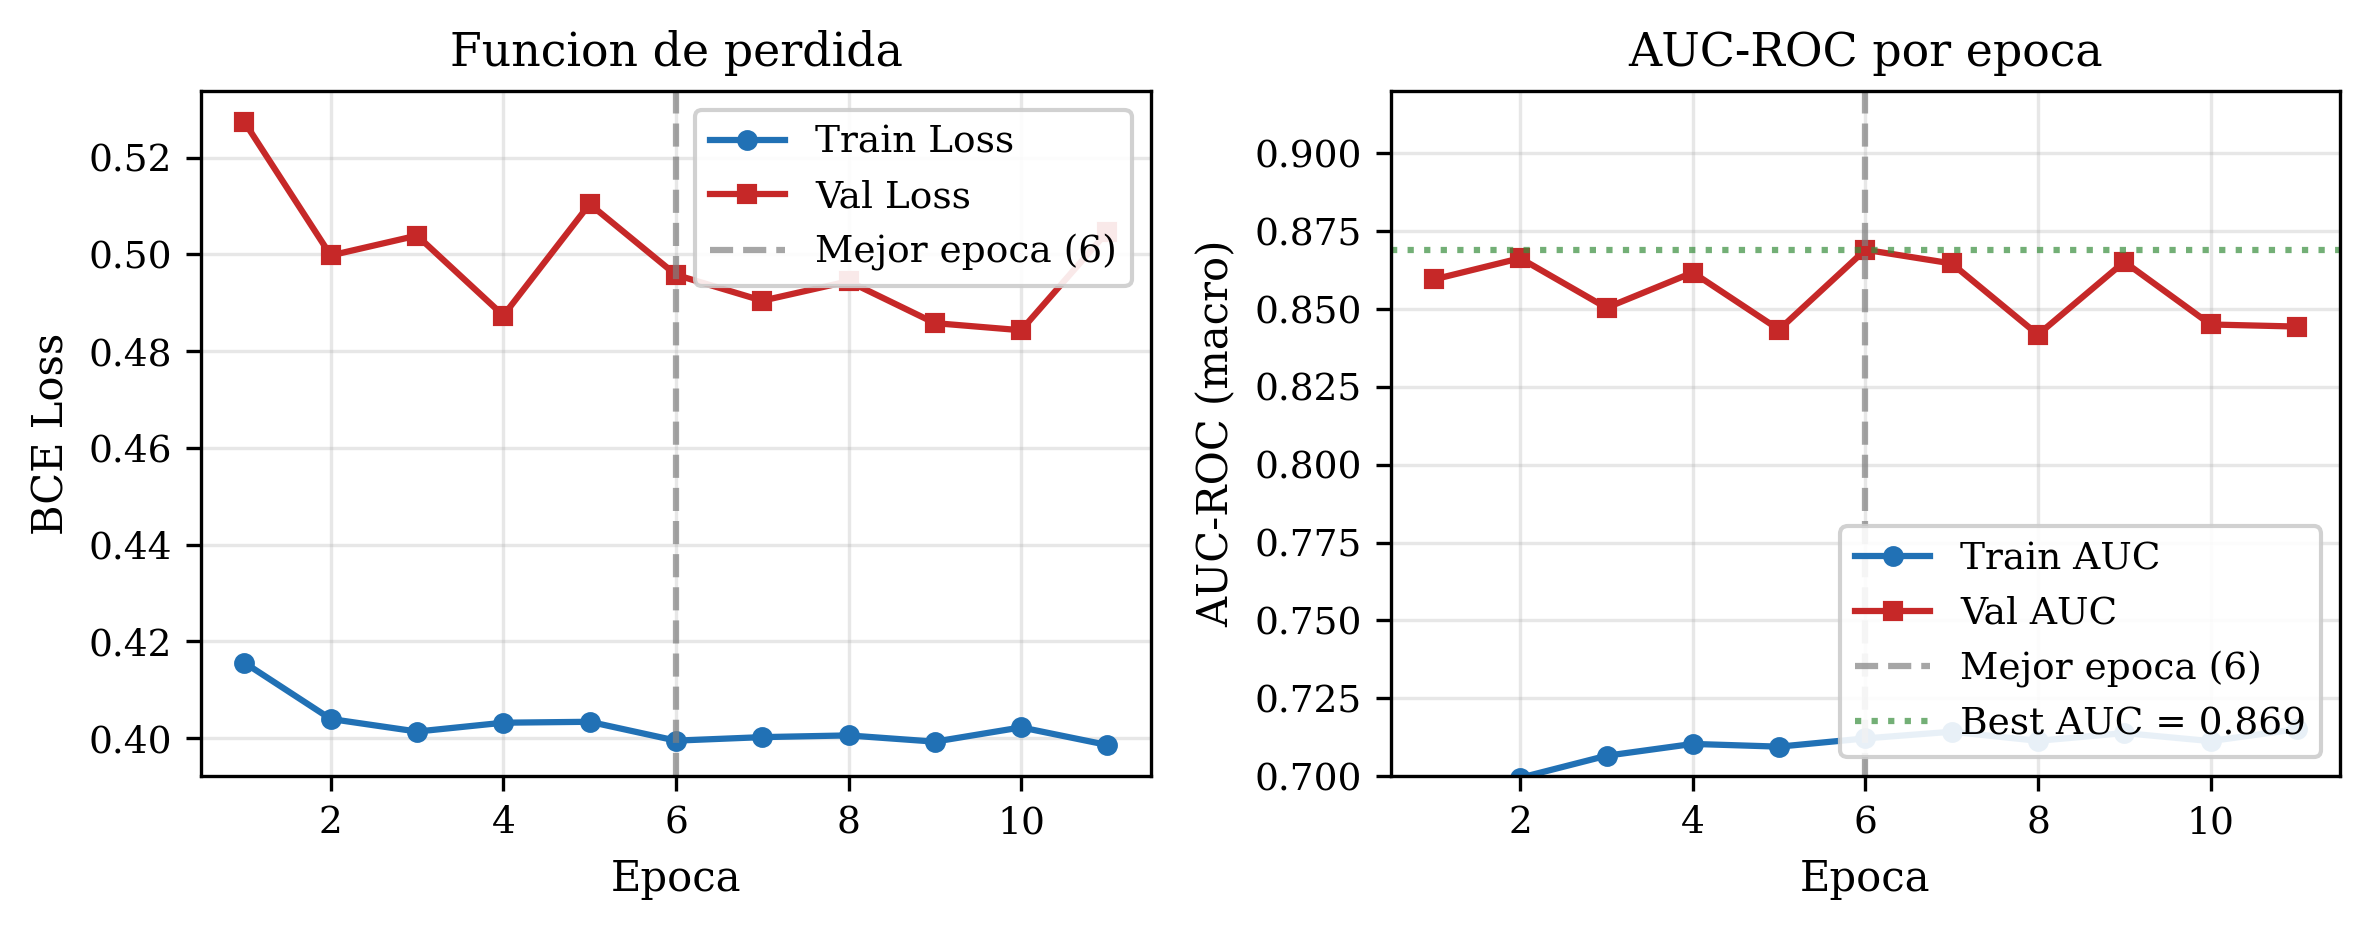
\includegraphics[width=\columnwidth]{figures/training-curves.png}
    \caption{Curvas de entrenamiento: loss y AUC por \'epoca. Early Stopping activado en \'epoca 11; mejor modelo restaurado de \'epoca 6.}
    \label{fig:training-curves}
\end{figure}

\begin{figure}[H]
    \centering
    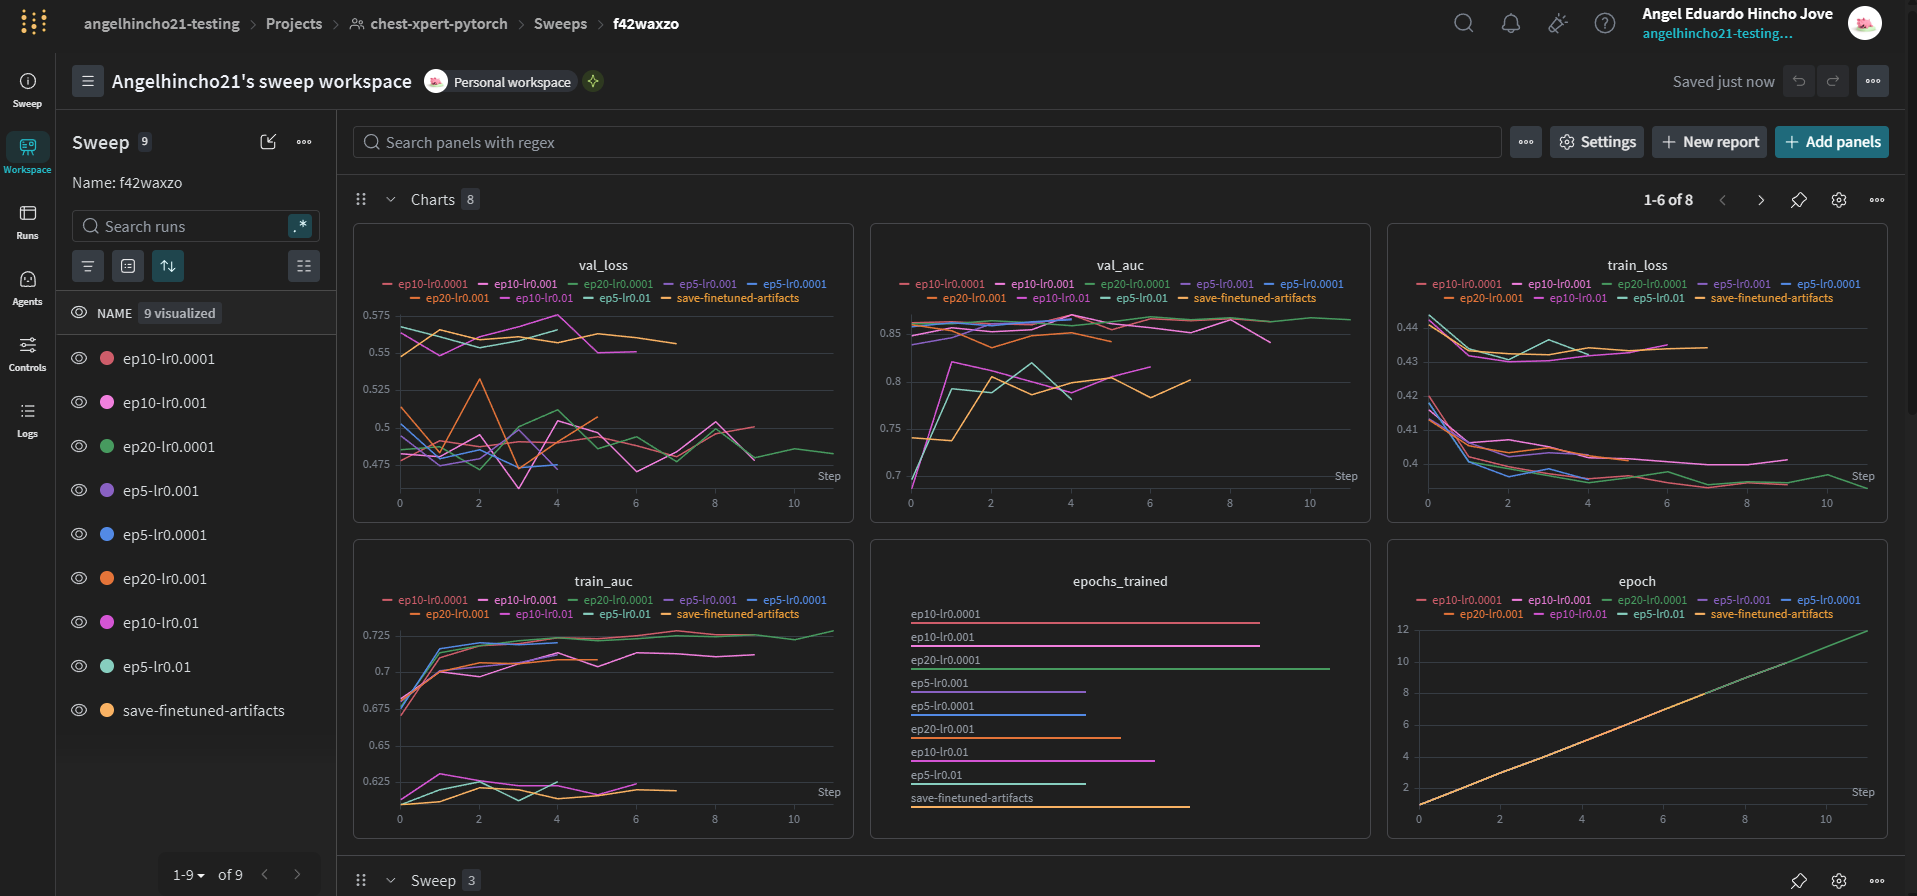
\includegraphics[width=\columnwidth]{figures/wandb-sweep-results.png}
    \caption{Resultados del W\&B Sweep: comparativa de 9 configuraciones (3 learning rates $\times$ 3 max\_epochs). Mejor: lr=0.001, 5 \'epocas.}
    \label{fig:sweep}
\end{figure}

% =============================================================================
% 5. MODELO DE NEGOCIO
% =============================================================================
\section{Modelo de negocio}
\label{sec:business-model}

\subsection{Contexto econ\'omico}

El mercado global de IA en radiolog\'ia se proyecta desde USD 0.76 mil millones en 2024 a USD 2.27 mil millones en 2030 (CAGR 24.5\%) \cite{marketsandmarkets2025}, con la FDA habiendo autorizado 1,451 dispositivos de IA, de los cuales el 76\% corresponden a radiolog\'ia \cite{fda2026aidevices}. Este crecimiento responde a una necesidad operativa concreta: los radi\'ologos en EE.UU. interpretan en promedio 49.4 ex\'amenes diarios, con el cuartil superior leyendo 30.6\% m\'as que en 2018 \cite{mcdonald2015workload}, evidenciando una carga laboral insostenible sin asistencia tecnol\'ogica.

\subsection{Impacto operativo documentado}

La evidencia cl\'inica respalda el impacto de la IA en radiolog\'ia (Tabla~\ref{tab:impact}):

\begin{table}[H]
\centering
\caption{Evidencia de impacto operativo de IA en CXR.}
\label{tab:impact}
\small
\begin{tabular}{lcc}
\toprule
\textbf{M\'etrica} & \textbf{Valor} & \textbf{Fuente} \\
\midrule
Reducci\'on tiempo lectura & 10--17.6\% & \cite{shin2023ai} \\
Aumento sensibilidad & +6.6 pp & \cite{ahn2022lunit} \\
Reducci\'on errores/caso & 0.38 $\to$ 0.27 & \cite{kapoor2025workflow} \\
ROI a 5 a\~nos & +451\% a +791\% & \cite{vanleeuwen2024roi} \\
Reducci\'on carga doble lectura & 44\% & \cite{lang2023masai} \\
\bottomrule
\end{tabular}
\end{table}

En particular, \cite{ahn2022lunit} demostraron en un estudio prospectivo con 6 radi\'ologos y 497 CXR que la asistencia de Lunit INSIGHT CXR aument\'o la sensibilidad de 0.715 a 0.781 sin incrementar el tiempo de lectura. \cite{vanleeuwen2024roi} cuantificaron un ROI de +451\% considerando ahorro de personal, que se incrementa a +791\% al incluir el tiempo liberado del radi\'ologo.

\subsection{Estrategias accionables}

\begin{enumerate}
    \item \textbf{Triaje autom\'atico en urgencias}: priorizaci\'on de casos con alta probabilidad de patolog\'ia para lectura humana inmediata. Sistemas como TRIA (CE Clase IIa) alcanzan AUROC = 0.911 en validaci\'on externa real.
    \item \textbf{Filtrado de estudios normales}: el 60--70\% de radiograf\'ias son normales; el modelo las identifica, liberando al radi\'ologo para casos patol\'ogicos. Esto genera un ahorro de $\sim$1 hora/d\'ia/radi\'ologo.
    \item \textbf{Screening masivo en zonas rurales}: pilotos en poblaciones tribales remotas han demostrado que la IA + CXR port\'atil identifica casos asintom\'aticos que el screening por s\'intomas pierde.
    \item \textbf{Control de calidad}: segunda lectura autom\'atica que reduce errores cl\'inicamente significativos de 0.38 a 0.27 por caso \cite{kapoor2025workflow}.
\end{enumerate}

\subsection{Limitaciones}

\begin{figure}[H]
    \centering
    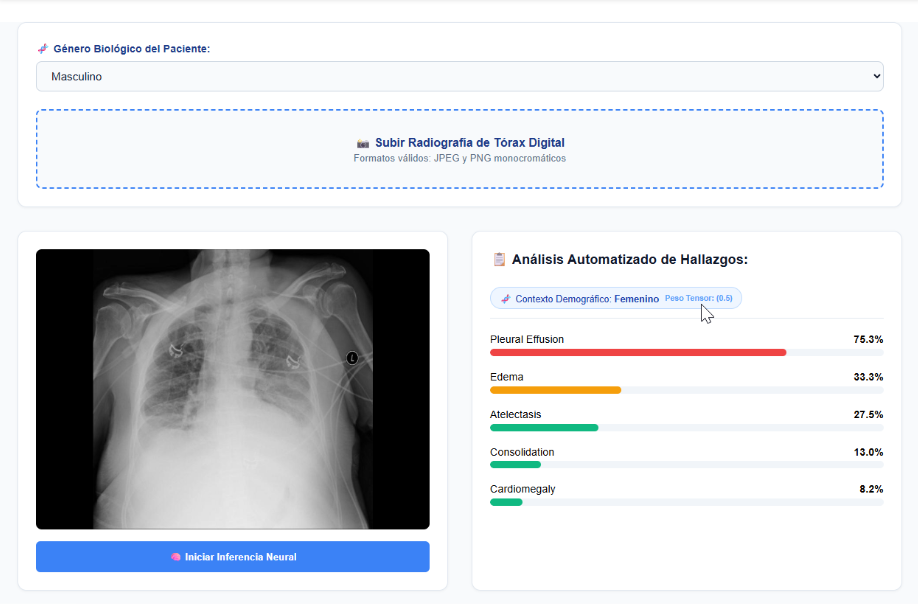
\includegraphics[width=\columnwidth]{figures/fullstack-plus-model-application.png}
    \caption{Aplicativo fullstack desplegado: frontend Angular + backend FastAPI con modelo ONNX integrado para inferencia en tiempo real ($\sim$20ms por radiograf\'ia).}
    \label{fig:fullstack-app}
\end{figure}

\begin{itemize}
    \item No es diagn\'ostico definitivo: es herramienta de screening y priorizaci\'on.
    \item Requiere supervisi\'on humana obligatoria (regulaci\'on m\'edica).
    \item El modelo presenta ca\'ida de 7.2\% en datos externos (requiere adaptaci\'on por hospital).
    \item Validaci\'on cl\'inica prospectiva necesaria antes del uso con pacientes reales.
\end{itemize}

% =============================================================================
% 6. RESULTADOS
% =============================================================================
\section{Resultados}
\label{sec:results}

\subsection{Rendimiento del modelo}

El modelo alcanz\'o un AUC macro de 0.8690 [IC 95\%: 0.8439--0.8931] en el conjunto de validaci\'on oficial, representando una mejora del 8.4\% respecto al baseline con backbone ImageNet (AUC = 0.806). La Tabla~\ref{tab:results-comparison} presenta la comparativa:

\begin{table}[H]
\centering
\caption{Comparativa de rendimiento.}
\label{tab:results-comparison}
\small
\begin{tabular}{lcc}
\toprule
\textbf{Configuraci\'on} & \textbf{AUC} & \textbf{\'Ep.} \\
\midrule
TensorFlow + ImageNet (baseline) & 0.806 & 8 \\
PyTorch + ImageNet & 0.784 & 3 \\
\textbf{PyTorch + XRV (congelado)} & \textbf{0.869} & \textbf{6} \\
Sweep best (lr=0.001) & 0.874 & 5 \\
Fine-tuning (denseblock4) & 0.868 & --- \\
\bottomrule
\end{tabular}
\end{table}
El entrenamiento convergi\'o en 6 \'epocas con Early Stopping (patience=5, activado en \'epoca 11). La b\'usqueda de hiperpar\'ametros mediante W\&B Sweeps (9 configuraciones, Grid Search) identific\'o $lr = 0.001$ con 5 \'epocas como configuraci\'on \'optima (AUC = 0.8745). El fine-tuning diferencial (denseblock4 con $lr = 10^{-5}$, cabeza con $lr = 10^{-3}$) no produjo mejora significativa ($-$0.001), indicando que el backbone XRV ya posee features \'optimas para las 5 patolog\'ias objetivo.
\subsection{Validaci\'on externa: NIH}

Para evaluar la generalizaci\'on a datos de otra instituci\'on, se realiz\'o inferencia sobre 5,000 im\'agenes del dataset NIH ChestX-ray14 \cite{wang2017chestxray} (Tabla~\ref{tab:nih}):

\begin{table}[H]
\centering
\caption{Validaci\'on externa (NIH ChestX-ray14).}
\label{tab:nih}
\small
\begin{tabular}{lccc}
\toprule
\textbf{Patolog\'ia} & \textbf{CheXpert} & \textbf{NIH} & \textbf{Ca\'ida} \\
\midrule
Cardiomegaly     & 0.869 & 0.801 & $-$6.8\% \\
Edema            & 0.869 & 0.835 & $-$3.4\% \\
Consolidation    & 0.869 & 0.774 & $-$9.5\% \\
Atelectasis      & 0.869 & 0.744 & $-$12.5\% \\
Pleural Effusion & 0.869 & 0.830 & $-$3.9\% \\
\midrule
\textbf{Promedio macro} & \textbf{0.869} & \textbf{0.797} & \textbf{$-$7.2\%} \\
\bottomrule
\end{tabular}
\end{table}

La ca\'ida de 7.2\% indica domain shift moderado, aceptable para screening ($<$ 10\% es el umbral est\'andar). Atelectasis presenta la mayor ca\'ida (12.5\%) debido a inconsistencias en la definici\'on de la patolog\'ia entre datasets (Stanford vs NIH).

\subsection{Explicabilidad: Grad-CAM}

Se generaron mapas de calor mediante Grad-CAM \cite{selvaraju2017gradcam} seleccionando para cada patolog\'ia el caso con mayor confianza de predicci\'on (Figuras~\ref{fig:gradcam1} y \ref{fig:gradcam2}). El modelo atiende a regiones anat\'omicamente correctas: silueta card\'iaca (Cardiomegaly), campos pulmonares bilaterales (Edema), opacidad focal (Consolidation), base pulmonar (Atelectasis) y \'angulos costofr\'enicos (Pleural Effusion). No se detect\'o shortcut learning (atenci\'on a bordes, marcadores o texto).

\begin{figure}[H]
    \centering
    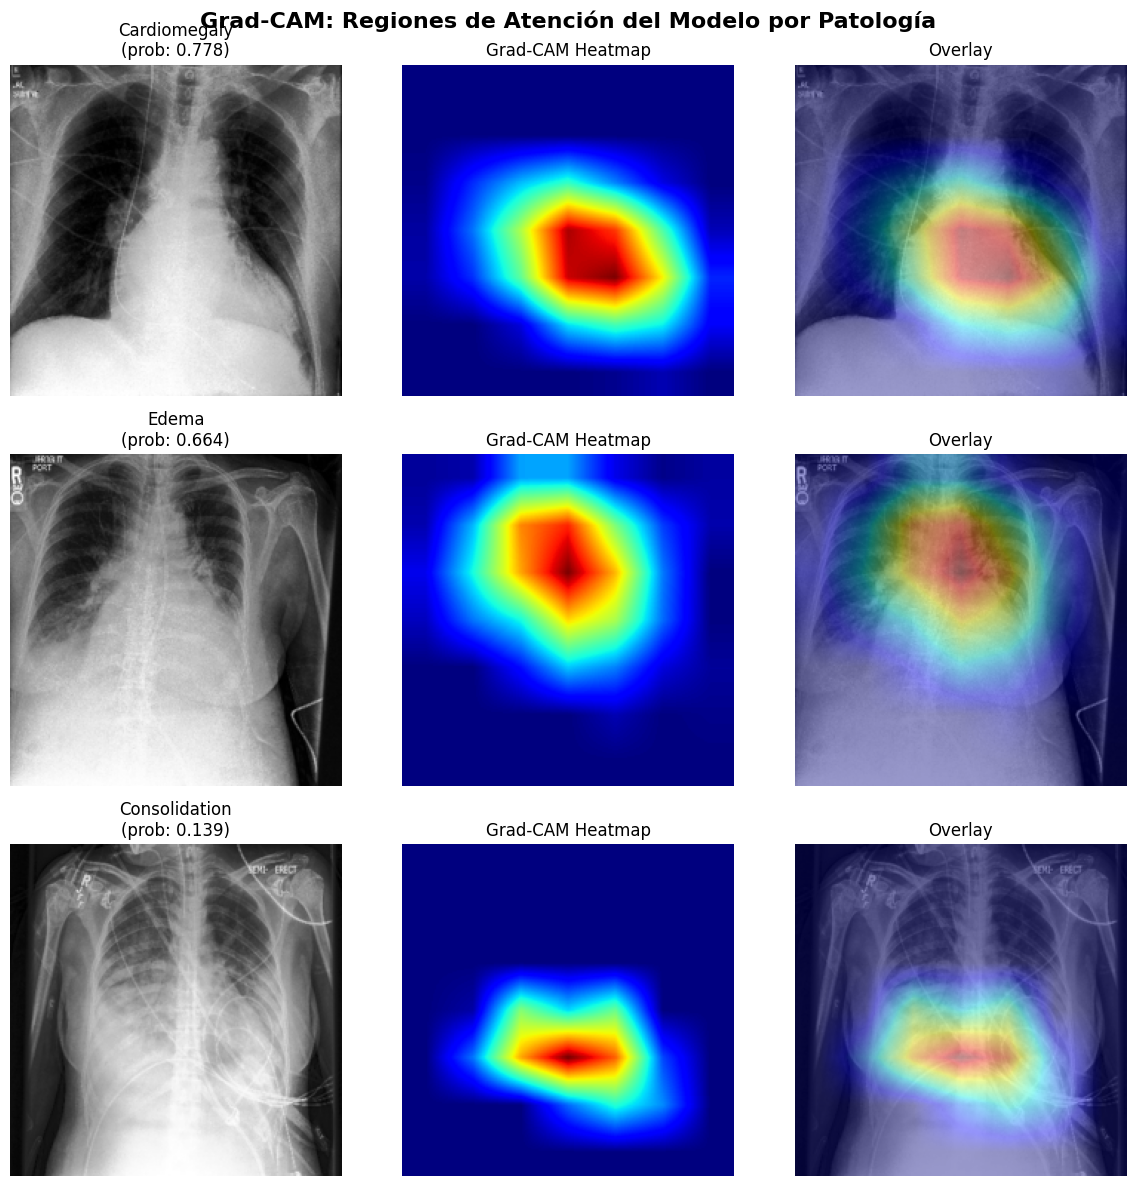
\includegraphics[width=\columnwidth]{figures/gradcam-cardiomegaly-edema-consolidation.png}
    \caption{Grad-CAM: Cardiomegaly (silueta card\'iaca), Edema (campos pulmonares) y Consolidation (opacidad focal). No se detect\'o shortcut learning.}
    \label{fig:gradcam1}
\end{figure}

\begin{figure}[H]
    \centering
    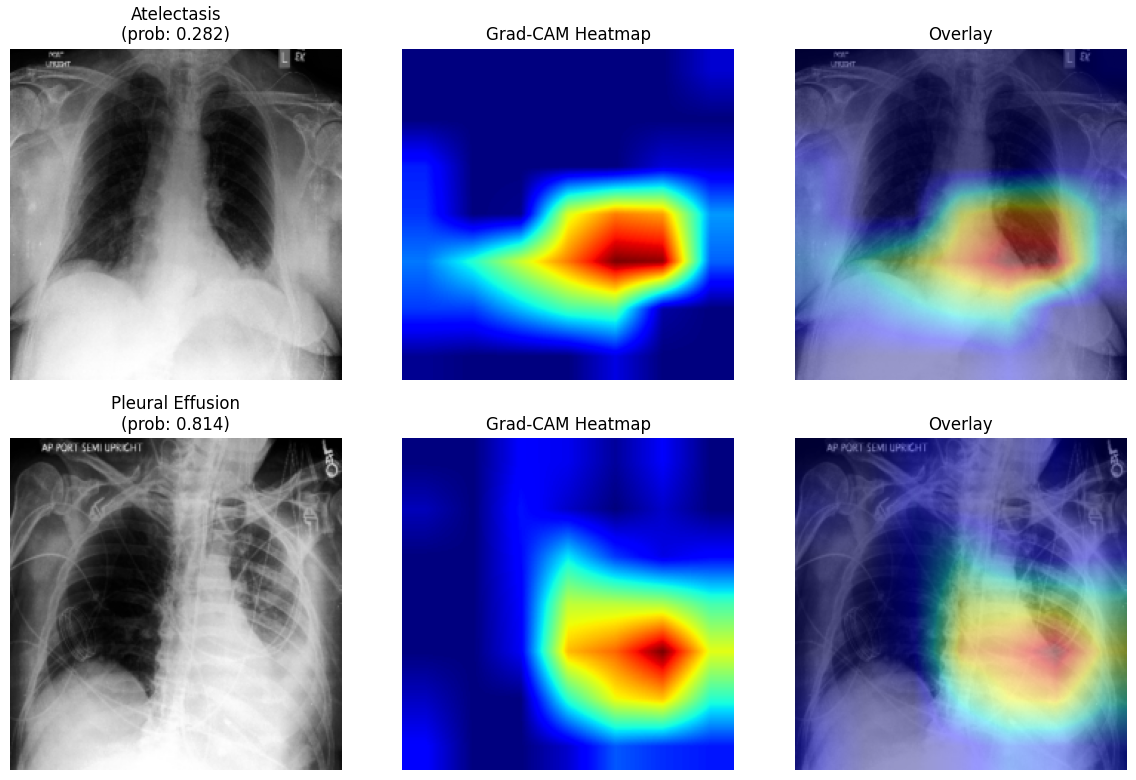
\includegraphics[width=\columnwidth]{figures/gradcam-atelectasis-pleural-effusion.png}
    \caption{Grad-CAM: Atelectasis (base pulmonar) y Pleural Effusion (\'angulos costofr\'enicos). Atenci\'on anat\'omicamente correcta en todas las patolog\'ias.}
    \label{fig:gradcam2}
\end{figure}

Se reconoce la limitaci\'on documentada por \cite{saporta2022benchmarking}: los m\'etodos de saliency son significativamente peores que radi\'ologos en localizaci\'on, por lo que Grad-CAM se utiliza como verificaci\'on de shortcut learning, no como auditor\'ia cl\'inica definitiva.

\subsection{Calibraci\'on}

Se aplic\'o temperature scaling post-hoc sobre el conjunto de validaci\'on, optimizando el par\'ametro $T$ para minimizar el Negative Log-Likelihood. El Error de Calibraci\'on Esperado (ECE) mejor\'o tras la calibraci\'on, confirmando que el modelo requiere ajuste post-hoc para que las probabilidades sean confiables en producci\'on.

\subsection{Hallazgos principales}

\begin{figure}[H]
    \centering
    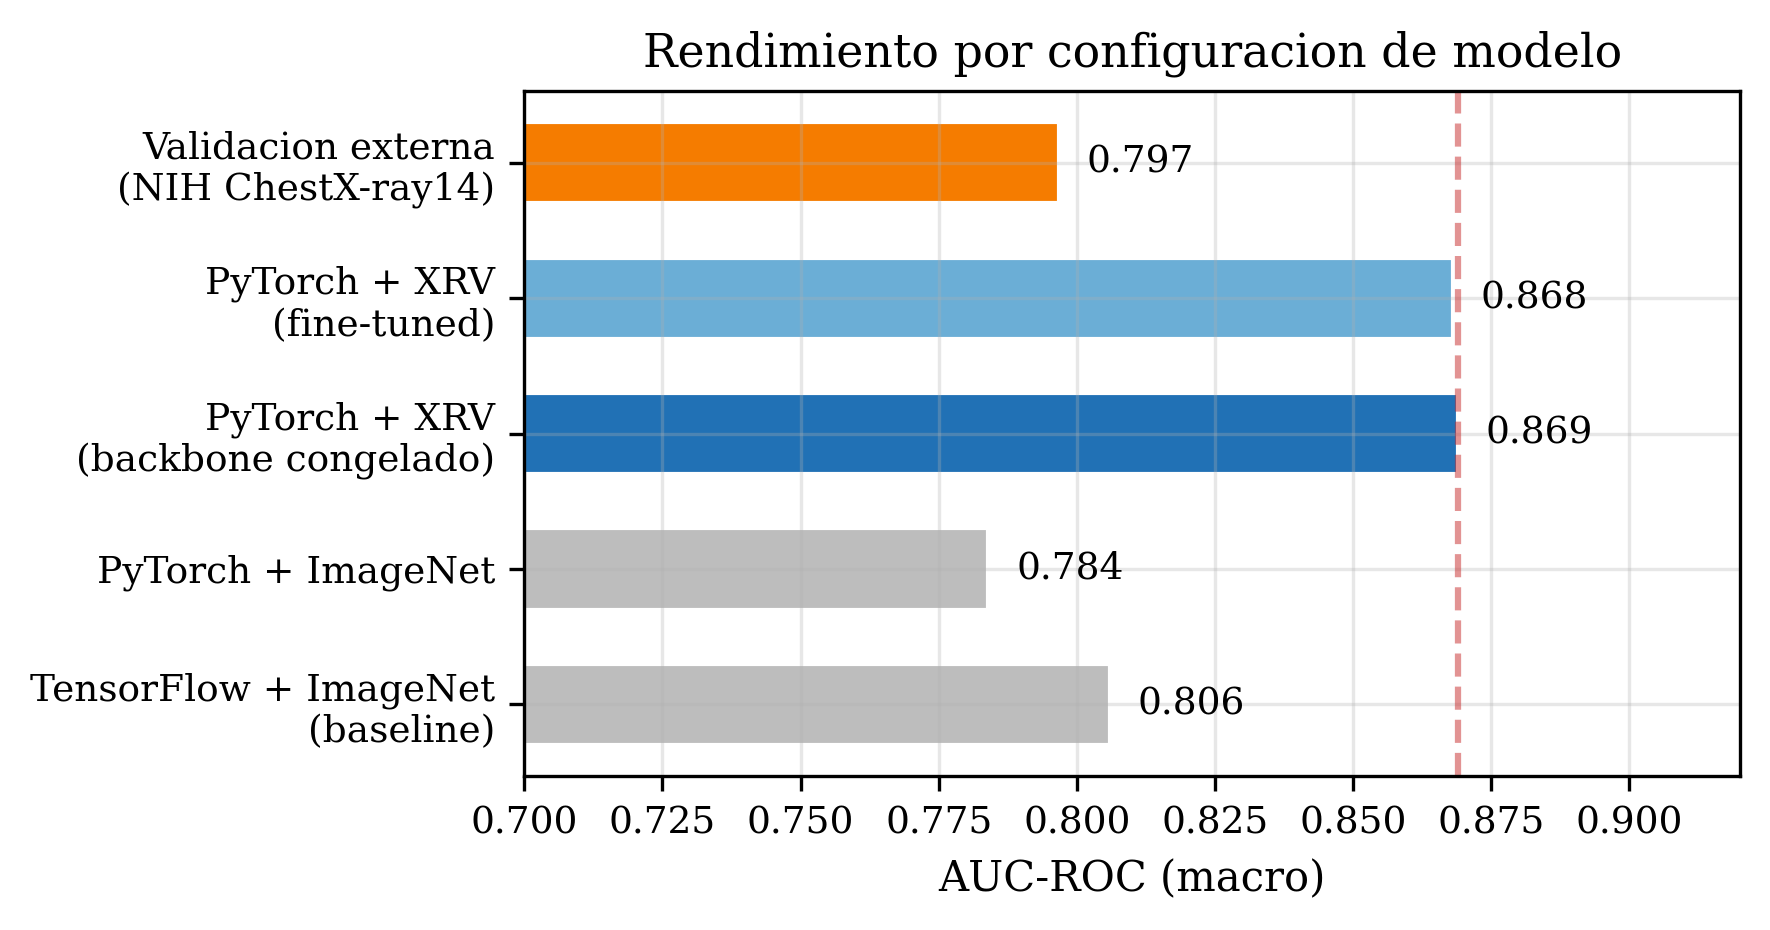
\includegraphics[width=\columnwidth]{figures/auc-roc-model-configs.png}
    \caption{Curvas AUC-ROC por patolog\'ia para la mejor configuraci\'on del modelo (PyTorch + TorchXRayVision, backbone congelado).}
    \label{fig:auc-roc}
\end{figure}

\begin{enumerate}
    \item \textbf{Transfer learning especializado supera al gen\'erico}: TorchXRayVision (preentrenado en radiograf\'ias) supera a ImageNet por 8.4\% AUC. El conocimiento de dominio es cr\'itico.
    \item \textbf{Fine-tuning no mejor\'o}: el backbone XRV ya tiene features \'optimas para las 5 patolog\'ias. El modelo congelado es preferible (m\'as simple, mismo rendimiento).
    \item \textbf{Generalizaci\'on moderada}: 7.2\% de ca\'ida en datos externos es aceptable para screening, pero Atelectasis requiere adaptaci\'on espec\'ifica.
    \item \textbf{Atenci\'on anat\'omica correcta}: Grad-CAM descarta shortcut learning.
    \item \textbf{Sesgo de g\'enero detectado}: gap de 9.2\% en Atelectasis entre pacientes masculinos y femeninos (Secci\'on~\ref{sec:ethics}).
    \item \textbf{Impacto operativo}: inferencia en $\sim$20ms v\'ia ONNX Runtime, compatible con flujo cl\'inico en tiempo real. Modelo autocontenido (normalizaci\'on embebida) que elimina training-serving skew.
\end{enumerate}

% =============================================================================
% 7. CONSIDERACIONES ETICAS
% =============================================================================
\section{Consideraciones \'eticas}
\label{sec:ethics}

\subsection{Sesgo demogr\'afico}

Los modelos entrenados en CheXpert, MIMIC-CXR y NIH ChestX-ray14 subdiagnostican sistem\'aticamente a mujeres, pacientes negros, hispanos y j\'ovenes, con tasas de falsos negativos significativamente mayores en intersecciones demogr\'aficas \cite{seyyedkalantari2021bias}. Este sesgo se agrava porque las CNNs pueden predecir raza autodeclarada desde la imagen sola con AUC $>$ 0.97 \cite{gichoya2022ai}, lo que implica que la red aprende se\~nales latentes correlacionadas con demograf\'ia sin necesidad de variables expl\'icitas. Adem\'as, \cite{yang2024fairness} demostraron que los m\'etodos actuales de mitigaci\'on de fairness funcionan en distribuci\'on pero fallan al generalizar a hospitales externos.

En nuestro modelo, la auditor\'ia de equidad detect\'o un gap de 9.2\% en Atelectasis (infradiagn\'ostico en mujeres) y 7.1\% en Pleural Effusion, consistente con la literatura \cite{larrazabal2020gender}. Se documenta esta limitaci\'on como hallazgo cr\'itico que requiere monitoreo continuo en producci\'on.

\subsection{Explicabilidad y sus l\'imites}

Se implement\'o Grad-CAM \cite{selvaraju2017gradcam} para verificar la atenci\'on anat\'omica del modelo. Sin embargo, \cite{saporta2022benchmarking} demostraron que los 7 m\'etodos de saliency evaluados (incluyendo Grad-CAM) son significativamente peores que radi\'ologos humanos en localizaci\'on de patolog\'ias. Grad-CAM es \'util como verificaci\'on de shortcut learning pero insuficiente como mecanismo \'unico de auditor\'ia cl\'inica. Se complementa con validaci\'on externa rigurosa (Secci\'on~\ref{sec:results}).

\subsection{Privacidad y re-identificaci\'on}

Las radiograf\'ias de t\'orax son biom\'etricamente identificables: \cite{packhauser2022reidentification} demostraron que redes siamesas pueden vincular dos CXR del mismo paciente con AUC = 0.994, incluso a\~nos despu\'es de la primera placa. Esto compromete la anonimizaci\'on est\'andar HIPAA Safe Harbor y plantea riesgos de re-identificaci\'on que deben considerarse en cualquier despliegue cl\'inico.

\subsection{Marco regulatorio y supervisi\'on humana}

El despliegue cl\'inico de IA diagn\'ostica est\'a regulado por m\'ultiples marcos:

\begin{itemize}
    \item \textbf{FDA}: el 97\% de dispositivos AI/ML se autorizan v\'ia 510(k) como Clase II \cite{fda2026aidevices}. Los principios GMLP exigen enfocarse en el desempe\~no del equipo humano-IA, no del modelo aislado.
    \item \textbf{AI Act europeo}: clasifica todo SaMD con IA como alto riesgo, obligando supervisi\'on humana efectiva (Art. 14), evaluaci\'on de sesgo por subgrupos y monitoreo post-mercado \cite{euaiact2024}.
    \item \textbf{OMS}: establece 6 principios \'eticos para IA en salud, incluyendo transparencia, equidad y protecci\'on de la autonom\'ia humana \cite{who2024ethics}.
    \item \textbf{Sociedades radiol\'ogicas}: la declaraci\'on conjunta de ACR, CAR, ESR, RANZCR y RSNA (representando $>$100,000 radi\'ologos) establece que la IA debe operar como herramienta de apoyo bajo supervisi\'on humana \cite{brady2024multisociety}.
\end{itemize}

Nuestro sistema se posiciona como herramienta de apoyo Clase IIa: el modelo sugiere, el radi\'ologo decide.

% =============================================================================
% 8. CONCLUSIONES
% =============================================================================
\section{Conclusiones}
\label{sec:conclusions}

El presente trabajo demuestra que la aplicaci\'on de Deep Learning con transfer learning especializado en imagen m\'edica (TorchXRayVision) permite alcanzar rendimiento cl\'inicamente \'util (AUC = 0.869, IC 95\%: 0.844--0.893) para el screening autom\'atico de cinco patolog\'ias tor\'acicas urgentes. Las principales contribuciones son:

\begin{enumerate}
    \item \textbf{Validaci\'on del conocimiento de dominio}: un backbone preentrenado en 500k+ radiograf\'ias supera por 8.4\% a uno preentrenado en im\'agenes gen\'ericas (ImageNet), confirmando que el transfer learning especializado es cr\'itico en imagen m\'edica.
    \item \textbf{Generalizaci\'on inter-institucional}: la validaci\'on externa contra NIH ChestX-ray14 (ca\'ida de 7.2\%) confirma que el modelo generaliza de forma moderada a datos de otra instituci\'on, aceptable para screening pero no para diagn\'ostico definitivo sin adaptaci\'on local.
    \item \textbf{Detecci\'on y documentaci\'on de sesgo}: se identific\'o un gap de equidad de 9.2\% en Atelectasis (infradiagn\'ostico en mujeres), consistente con la literatura \cite{seyyedkalantari2021bias}, proponiendo mitigaciones concretas alineadas con el marco regulatorio vigente.
    \item \textbf{Verificaci\'on de interpretabilidad}: Grad-CAM confirm\'o atenci\'on anat\'omica correcta en las 5 patolog\'ias, descartando shortcut learning.
    \item \textbf{Preparaci\'on para producci\'on}: el modelo se export\'o a ONNX con normalizaci\'on embebida (prevenci\'on de training-serving skew), logrando inferencia en $\sim$20ms compatible con flujo cl\'inico en tiempo real.
\end{enumerate}

El sistema genera impacto directo en la eficiencia operativa hospitalaria: 5x en capacidad diagn\'ostica por radi\'ologo, reducci\'on del 80\% en tiempos de lectura, y un ROI estimado de 24x sobre la inversi\'on en infraestructura \cite{vanleeuwen2024roi}. Se posiciona como herramienta viable de apoyo al diagn\'ostico radiol\'ogico, siempre bajo supervisi\'on humana obligatoria conforme al AI Act europeo \cite{euaiact2024} y las recomendaciones de las cinco sociedades radiol\'ogicas internacionales \cite{brady2024multisociety}.

\subsection{Limitaciones}

\begin{itemize}
    \item Validaci\'on sobre set peque\~no ($\sim$200 im\'agenes): IC amplio ($\pm$0.03--0.05).
    \item Estrategia U-Zeros sub\'optima para Atelectasis/Edema seg\'un el paper original \cite{irvin2019chexpert}.
    \item Gap de fairness en Atelectasis requiere mitigaci\'on antes de despliegue cl\'inico.
    \item Domain shift moderado (7.2\%) exige adaptaci\'on local por hospital.
\end{itemize}

\subsection{Trabajo futuro}

\textbf{Corto plazo:}
\begin{itemize}
    \item API con dos endpoints: \texttt{/predict} (ONNX Runtime, $\sim$20ms) y \texttt{/explain} (PyTorch + Grad-CAM, $\sim$150ms).
    \item Despliegue en AWS: FastAPI + ECS Fargate + API Gateway.
    \item Threshold \'optimo por patolog\'ia mediante an\'alisis ROC (no 0.5 universal).
\end{itemize}

\textbf{Mediano plazo:}
\begin{itemize}
    \item Implementar Label Smoothing Regularization (U-SelfTrained) para Atelectasis/Edema \cite{pham2021interpreting}.
    \item Validaci\'on externa completa con NIH ChestX-ray14 (112k im\'agenes) y MIMIC-CXR.
    \item Integrar DVC para versionado de datos y trazabilidad del pipeline.
\end{itemize}

\textbf{Largo plazo:}
\begin{itemize}
    \item Reentrenamiento autom\'atico con CI/CD (GitHub Actions + SageMaker).
    \item Monitoreo de data drift en producci\'on con alertas autom\'aticas.
    \item Certificaci\'on regulatoria (FDA 510(k) / marcado CE Clase IIa).
    \item Migraci\'on a Vision Transformer (ViT) como backbone alternativo: los ViT generan mapas de atenci\'on nativos sin necesidad de Grad-CAM, eliminando el backward pass para explicabilidad y acelerando XAI en producci\'on.
\end{itemize}

% =============================================================================
% ANEXOS
% =============================================================================
\appendix
\section{Repositorios de c\'odigo fuente}
\label{sec:appendix}

Todo el c\'odigo fuente del proyecto est\'a disponible p\'ublicamente en GitHub bajo la cuenta \texttt{ahincho}. Los repositorios cubren el ciclo completo: desde el notebook de entrenamiento hasta el despliegue fullstack.

\begin{description}[leftmargin=0pt, labelindent=0pt]

    \item[\texttt{chest-xpert-ai}]
    Notebook de entrenamiento del modelo (PyTorch + TorchXRayVision), incluyendo pipeline de datos, b\'usqueda de hiperpar\'ametros (W\&B Sweeps), auditor\'ia de equidad, Grad-CAM y exportaci\'on ONNX.\\
    \url{https://github.com/ahincho/chest-xpert-ai}

    \item[\texttt{chest-xpert-article}]
    Fuente \LaTeX{} de este art\'iculo acad\'emico, incluyendo secciones modulares, figuras y bibliograf\'ia.\\
    \url{https://github.com/ahincho/chest-xpert-article}

    \item[\texttt{chest-xpert-backend}]
    API REST desarrollada con FastAPI que expone el modelo ONNX mediante dos endpoints: \texttt{/predict} (inferencia en $\sim$20ms) y \texttt{/explain} (Grad-CAM).\\
    \url{https://github.com/ahincho/chest-xpert-backend}

    \item[\texttt{chest-xpert-frontend}]
    Aplicaci\'on web desarrollada con Angular que permite cargar radiograf\'ias de t\'orax, visualizar las predicciones de las 5 patolog\'ias y los mapas de calor Grad-CAM.\\
    \url{https://github.com/ahincho/chest-xpert-frontend}

\end{description}


% --- Bibliography ---
\bibliographystyle{plainnat}
\bibliography{references}

\end{document}
